% This text is proprietary.
% It's a part of presentation made by myself.
% It may not used commercial.
% The noncommercial use such as private and study is free
% Dec 2007
% Author: Sascha Frank
% University Freiburg
% www.informatik.uni-freiburg.de/~frank/
%
%
\documentclass{beamer}
\usepackage{amsfonts}
\usepackage{amssymb,amsmath}
\usepackage{dsfont}
\usepackage{subfigure}


\setbeamertemplate{navigation symbols}{}
\setbeamercolor{frametitle}{fg=black,bg=white}
\setbeamercolor{title}{fg=black,bg=yellow!85!orange}
\usetheme{AnnArbor}
\beamersetuncovermixins{\opaqueness<1>{25}}{\opaqueness<2->{15}}
\DeclareMathOperator*{\argmax}{arg\,max\,}
\DeclareMathOperator*{\minimize}{minimize\,}
\DeclareMathOperator*{\argmin}{arg\,min\,}
\newcommand{\norm}[1]{\left \lVert #1 \right \rVert}
\newcommand{\normtwo}[1]{\left \lVert #1 \right \rVert_2^2}
\newcommand{\normf}[1]{\left \lVert #1 \right \rVert_{Fro}}

\DeclareSymbolFont{letters}{OML}{ztmcm}{m}{it}
\DeclareSymbolFontAlphabet{\mathnormal}{letters}
\SetSymbolFont{letters}{normal}{OML}{ztmcm}{m}{it}
\AtBeginSection[]
{
 \begin{frame}<beamer>
 \frametitle{Plan}
 \tableofcontents[currentsection]
 \end{frame}
}

%%%%%%%%%%%%%%%%%%%%%%%%%%%%%%%55
\begin{document}
\title{Deep Zero-Shot Learning}
\author{Seyed Mohsen Shojaee}
\date{}

\begin{frame}[plain, noframenumbering]
  \begin{center}
\begin{figure}

\includegraphics[scale=0.5]{../images/logo.pdf}
\end{figure}
{\footnotesize Sharif University of Technology \\ Computer Engineering Department \\ MSc Thesis}
\maketitle
\vspace{-10mm}{\footnotesize supervised by \\ Dr.Mahdieh Soleymani} \\
\vspace{4mm}
Summer 2016
\end{center}
\end{frame}



\begin{frame}
  \frametitle{Plan}
  \tableofcontents
\end{frame}


\section{Introduction}
\begin{frame}
  \frametitle{Introduction}
    \subsection{Standard Learning Paradigm}
    \textbf{Standard Supervised Learning Paradigm:}
    Discover the pattern for each class from abundant labeled samples.
    \begin{itemize}
      \item Using SVM, Decision Tree, KNN, etc.
    \end{itemize}
    \begin{figure}
    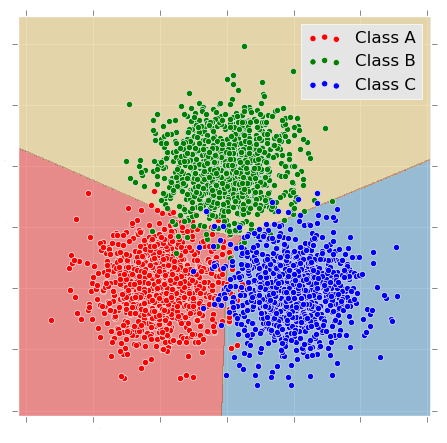
\includegraphics[width= 0.5\linewidth]{multi.png}
    \end{figure}
\end{frame}

\subsection{Zero-shot Learning definition}
\begin{frame}
  \frametitle{Extening the Standard Paradigm}
  Sometimes samples from all classes is not available
  \begin{itemize}
    \item Example: Novel Categories, Fine-grained classification.
  \end{itemize}

  \textbf{Zero-Shot Learning} addresses the problem of classification.
  \begin{itemize}
    \item[]  when no training sample is available for some classes.
  \end{itemize}
  \begin{figure}
  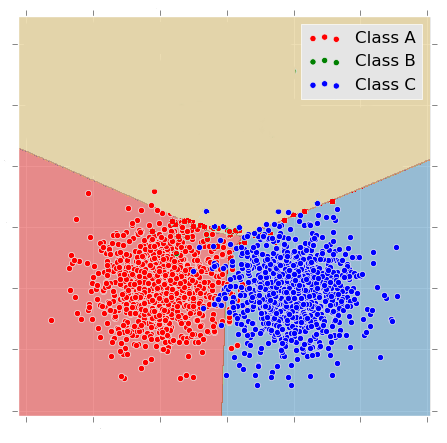
\includegraphics[width= 0.3\linewidth]{zero.png}
  \end{figure}
\end{frame}
\begin{frame}\frametitle{Extening the Standard Paradigm}
\textbf{Identifying Classes without Samples:}
\begin{itemize}
  \item Each category is identified some \textit{auxiliary information} also called
  \textit{signature}.
  \item Examples of class signatures include:
  \begin{itemize}
    \item Attribute Vectors
    \item Text Articles
    \item Category Names
  \end{itemize}
  \item Signatures exist for all classes.
\end{itemize}
\end{frame}
\begin{frame}\frametitle{Extening the Standard Paradigm}
    As a sample, an animal species like Zebra can have these signatures:
    \begin{columns}
    \begin{column}{7cm}
      \begin{itemize}
        \item The Vector (four legs, fast, striped, gallops, non-domestic, ...).
        \item The Wikipedia Entry for zebra.
        \item The word \textit{'Zebra'} itself.
      \end{itemize}
    \end{column}
    \begin{column}{5cm}
      \begin{figure}
      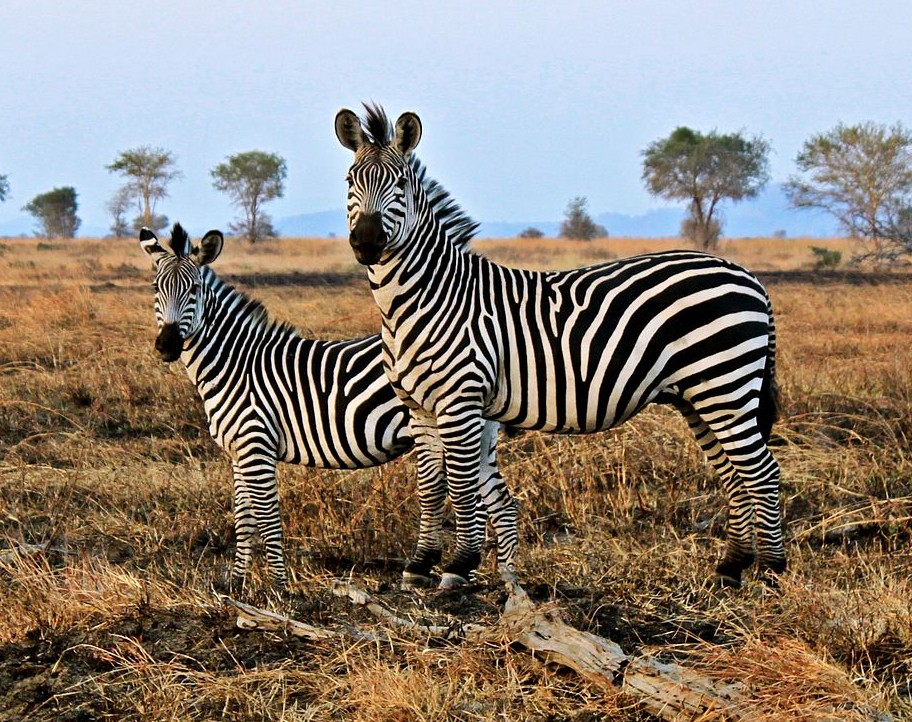
\includegraphics[width= 4cm]{zebra.jpg}
      \end{figure}
    \end{column}
\end{columns}
\end{frame}

\begin{frame}\frametitle{Problem Definition}
  \textbf{At training time:}
\begin{itemize}
  \item there are $N_s$ labeled samples:  $ \{ (\mathbf{x}_i, \mathbf{y}_i) \}_{i=1}^{N_s} $.
  \item These samples are from $n_s$ classes that are called \textit{seen classes}.
  \item Class signatures $C_s$ for seen classes is also available.
  \item There are also $n_u$ classes with no labeled sample. These are called \textit{unseen classes.}
  \item It is assumed in most works that signatures of unseen classes, $C_u$, is also available.
\end{itemize}
\end{frame}

\begin{frame}\frametitle{Problem Definition}
  \textbf{At test time:}
  \begin{itemize}
    \item  $N_u$ samples from unseen classes are presented: $ \{ (\mathbf{x}_i) \}_{i=N_s + 1}^{N_s + N_u} $.
    \item The Goal is to classify test samples into unseen categories.
    \item In other words finding
     $$ \argmin_{\mathbf{y^{\ast}}_i}  \mathbf{y^{\ast}}_i  \neq \mathbf{y}_i, \quad i= N_s +1 , \ldots, N_s + N_u $$
  \end{itemize}
\end{frame}

\subsection{Solution Steps}
\label{sub:Solution Steps}

\begin{frame}\frametitle{Solution Steps}
Most existing solutions for zero-shot learning consist of these three steps:
\begin{enumerate} \pause
\item Embed images in a semantic space \pause
\item Embed class signatures to same semantic space \pause
\item Assign images to those classes (e.g. using nearest neighbor classifier)
\end{enumerate}
\end{frame}
\section{Prior Works}
\subsection{A categorization of existing methods}
\label{sec:Prior Works}
\begin{frame}\frametitle{Prior Works}
  Existing works can be categorized by the semantic space they use:
  \begin{itemize}
    \item Space of signatures (Attribute Prediction).
    \item Space of images.
    \item A third space.
  \end{itemize}
  We review some selected works from each category.
\end{frame}
\subsubsection{Attribute Prediction}
\begin{frame}\frametitle{Attribute Prediction}
  \begin{itemize}
    \item A large body of work in zeroshot learning belongs to this category.
    \item The mapping from signature space is considered identity mapping.
    \item Attribute Estimator/Classifier are learned on train images (standard supervised problem).
    \item The Estimator/Classifier is used on test images to find $\mathbf{c}^{\ast}_i$ for image $\mathbf{x}_i$
    \item $\mathbf{x}_i$ is assigned to class with most similar signature:
    $$ \ell(\mathbf{x}_i) = \argmin_{j=n_s+1 \ldots, n_s + n_u} distance(\mathbf{c}^{\ast}_i, \mathbf{c}_j) $$
  \end{itemize}

  Examples from this category include: \cite{akata13,jayaraman14,lampert09}
\end{frame}

\subsubsection{Mapping to image space}
\begin{frame}
  \frametitle{Mapping to Image Space}
\begin{itemize}
    \item In training time, Learn a mapping from class signatures to image space:
    \[ \phi: \mathbb{R}^{a} \to \mathbb{R}^d \]
    \item This can bee seen predicting linear one-vs-all classifier for each class from its signature.
    \item In test time, classify test images using classifiers predicted from unseen class signatures.
    \item Assign each sample to class whose classifier produces maximum score:
    \begin{equation}
      \ell(\mathbf{x}) = \argmax_{j=n_s+1 \ldots, n_s + n_u} \langle \phi(\mathbf{c}_j), \mathbf{x} \rangle
    \end{equation}
\end{itemize}

Examples from this category include: \cite{elhoseiny2015,Reed2016}
\end{frame}

\subsubsection{Mapping to a middle space}
\begin{frame}
  \frametitle{Mapping to a middle Space}
\begin{itemize}
    \item In training time  mappings $ \theta(\mathbf{c})$ and $\phi(\mathbf{x})$ are learned.
    \item The mapping should map image $\mathbf{x}$ close to its true signature $\mathbf{c}$
    \item And with a margin from other signatures.
    \item In this way we expect $\theta$ and $\phi$ to map signature and samples of same unseen classes also close to each other. \pause
    \item Space of seen classes has been a successful choice for middle space \pause
    \item Bilinear mappings fall into this category too.
\end{itemize}
\pause
Examples from this category include: \cite{ba2015,Reed2016}
\end{frame}

\subsection{Semi-supervised Zero-shot Learning}
\label{sec:Semi-supervised Zero-shot Learning}
\begin{frame}\frametitle{Semi-supervised Zero-shot Learning}
\begin{itemize}
  \item Use Unsupervised information in structure of unlabeled images.
  \item This information helps finding better mappings \pause
  \item Semi-supervised methods can alleviate \textit{domain shift problem} by using unlabeled samples.
\end{itemize}
\vspace{1cm}
\pause
Examples include: \cite{semi15,li15max,Kodirov2015,Fu2014}
\end{frame}

\begin{frame}\frametitle{Domain shift problem}
  \begin{itemize}
    \item Attributes are represented with different visual features in different classes.
    \item Mapping Learned on seen classes would not do as good on unseen classes.
    \begin{figure}
      \centering
      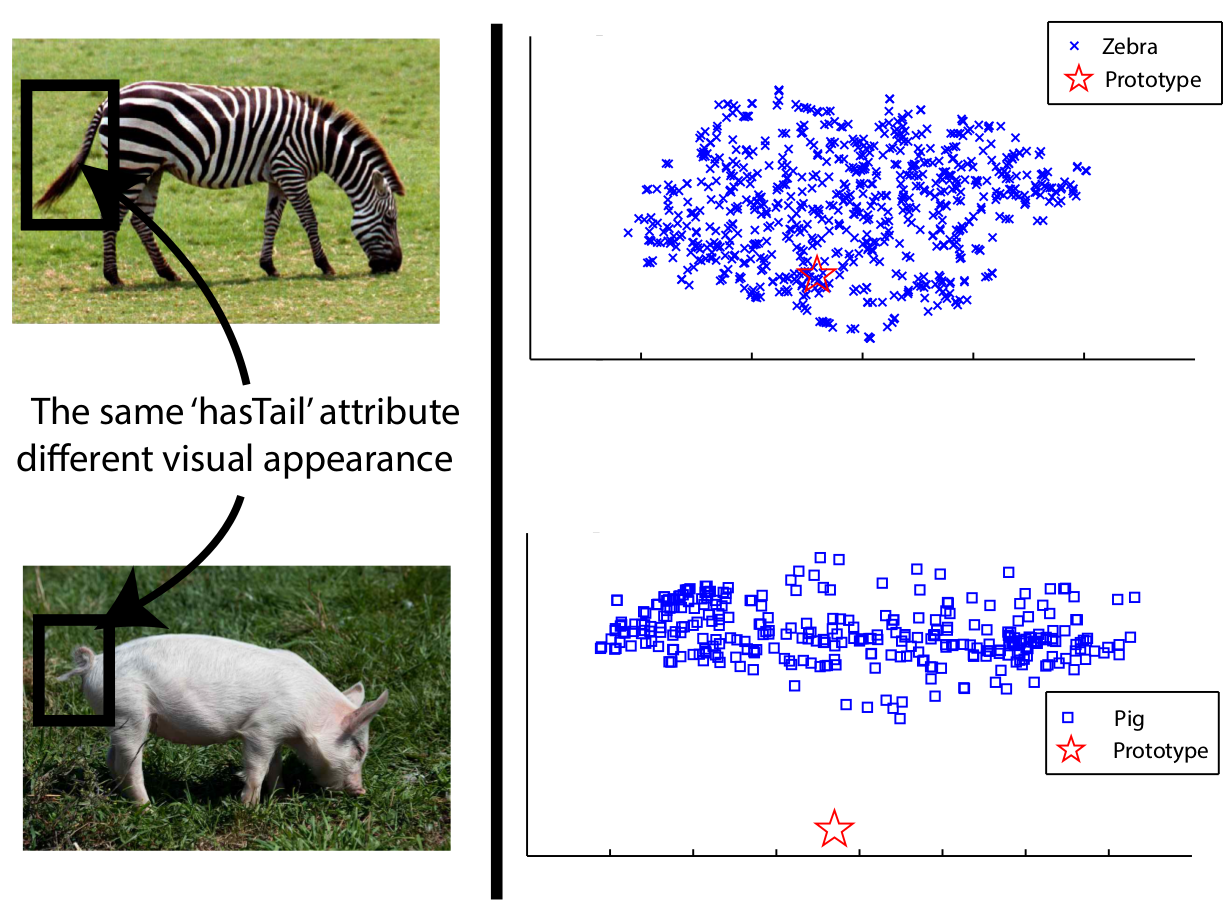
\includegraphics[width=6cm]{domain-shift.png}
      \caption{\scriptsize
      Different visual representation of attribute ``has tail'' \cite{Fu2014}.
      }
    \end{figure}
  \end{itemize}
\end{frame}


\section{Proposed Methods}
\begin{frame}\frametitle{Proposed Methods}
Here we present four proposed methods for the problem of zero-shot Image Classification.

In our methods we consider class signatures of type attribute vectors.

\begin{itemize}
  \item Attribute Prediction with Multi-task Deep Neural Networks.
  \item Mapping to Histograms of Seen Classes with Deep Neural Network.
  \item Independent Embedding and Clustering
  \item Joint Embedding and Clustering
\end{itemize}
\end{frame}

\subsection{Multi-task Neural Network}
\begin{frame}\frametitle{Multi-task Neural Network}
  We propose a network architecture for attribute prediction from images.

  The network:
\begin{itemize}
  \item  predicts for train and test images at the same time (hence multi-task).
  \item can mitigate the domain shift problem that appears when only samples from seen classes is used.
  \item uses 17 layers from famous VGG-19 network \cite{vgg}  for feature extraction.
  \item is trained fast using Stochastic gradient descent algorithms family.
\end{itemize}
\end{frame}

\begin{frame}\frametitle{Multi-task Neural Network}
\begin{itemize}
\item[] Let $f$ denote the mapping modeled by the multi-task network.
\item[] Then  $\mathbf{\hat{c}}_i = f (\mathbf{x}_i) $ would be attributes predicted by network for $\mathbf{x}_i$
\item[] We learn $f$ such that:
\end{itemize}
  \begin{equation}
\label{eq:nn_loss}
\minimize_{f}
\frac{1}{N_s} \sum_{i=1}^{N_s} loss(\mathbf{\hat{c}}_i, \mathbf{c}_{y_i}) +
\frac{\gamma}{N_u} \sum_{i=N_s}^{N_s+N_u} \Big ( \min_{j=n_s,\ldots,n_s + n_u} loss(\mathbf{\hat{c}_i , c_j}) \Big ).
\end{equation}
The second term enforces that prediction for test samples to be close to an unseen class signature

Therefore, mitigating domain-shift problem
\end{frame}

\begin{frame}\frametitle{Multi-task Neural Network}
  \begin{figure}
  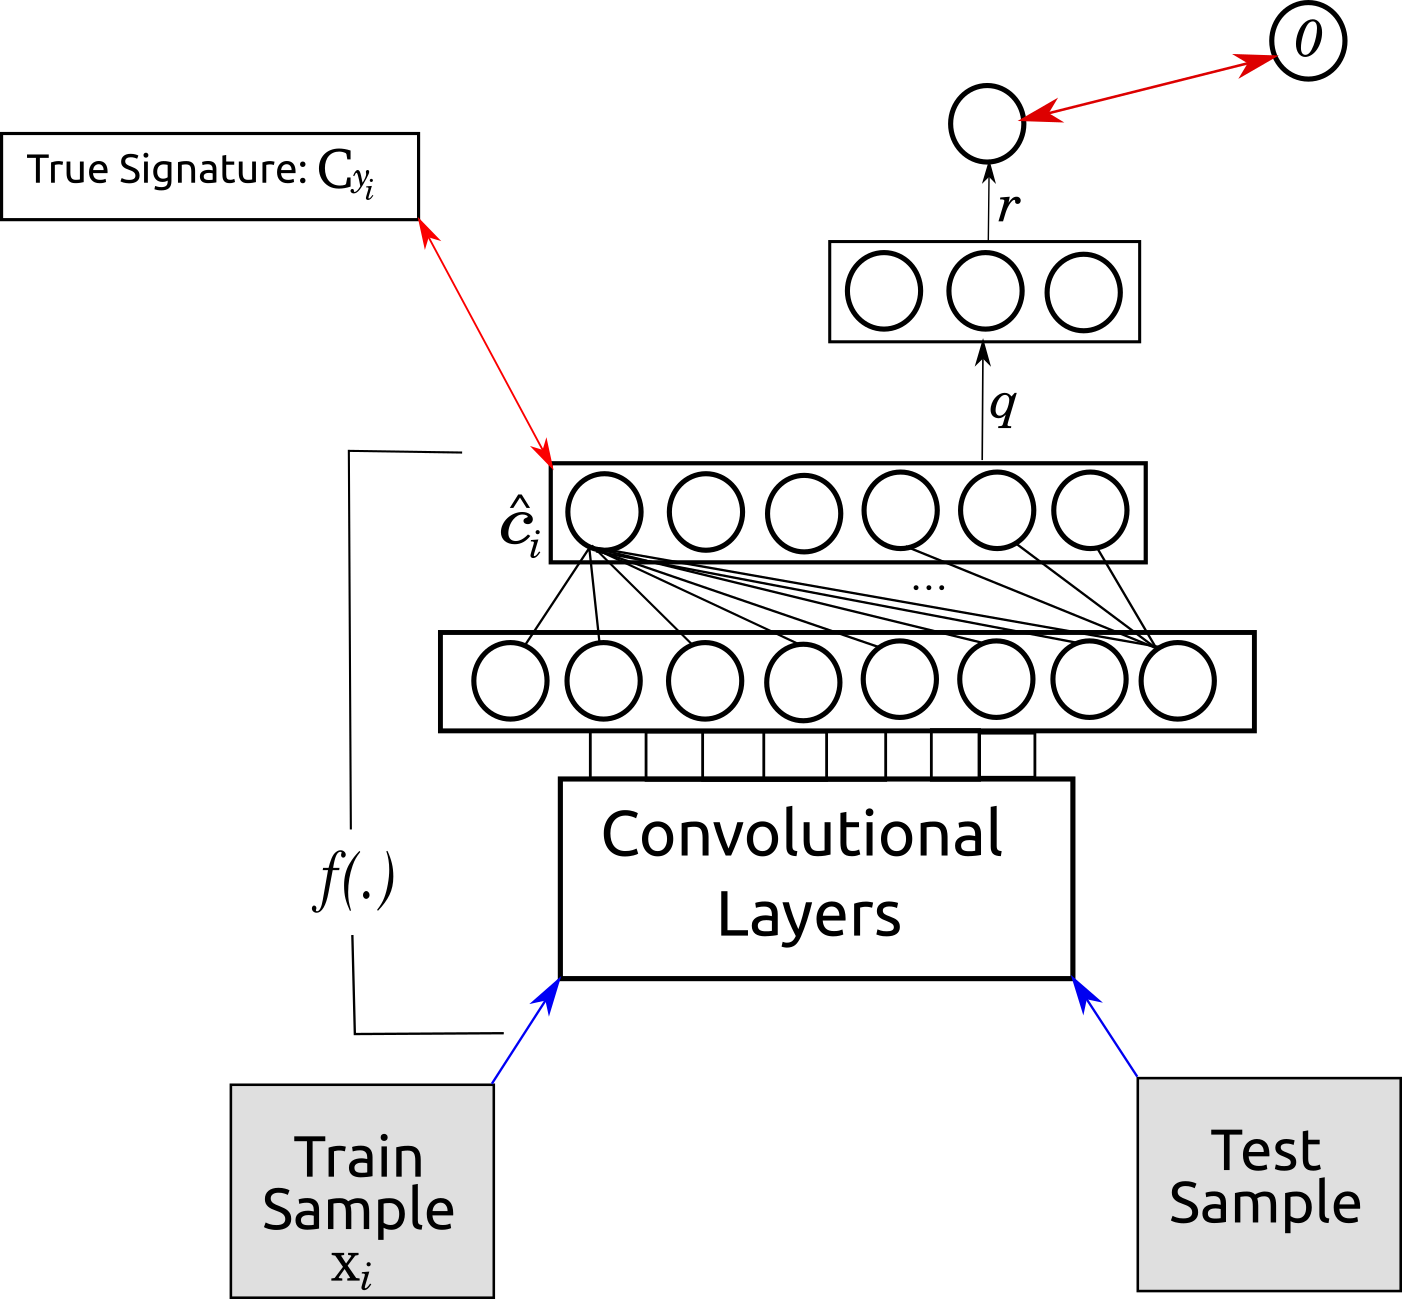
\includegraphics[scale=0.4]{net}
  \caption{Proposed Multi-task network Architecture}
  \end{figure}
\end{frame}

\begin{frame}\frametitle{Multi-task Neural Network}
The second term in Eq. \eqref{eq:nn_loss} is modeled by two layers, $q$ and $r$:
\begin{align}
\label{eq:min_layer}
\big(q(\mathbf{v})\big )_j &=  \normtwo{f(\mathbf{v) - c_j}}, \\
r(\mathbf{z}) &= \min_{j=1\ldots n_u} (\mathbf{z})_j.
\end{align}
\begin{itemize}
  \item The $j-$th element of $q$ shows distance of prediction made by network to signature of $j-$th unseen category.
  \item $r$ selects the minimum element of its input
  \item Hence using $q$ and $r$ successively produces distance of prediction to nearest unseen class signature.
  \item This is exactly same as the second term in Eq. \eqref{eq:nn_loss}
\end{itemize}
\end{frame}


\begin{frame}\frametitle{Comparison with other attribute prediction methods}
{\scriptsize
\begin{table}
  \caption{Multi-calss accuracy in form of average $\pm$ std}
\begin{tabular}{|l|c|c|c|c|}
\hline
method  & AwA & CUB-2011 & aPY & SUNA \\
\hline \hline
 {\tiny \cite{jayaraman14}}  & $43.01 \pm 0.07$ &        -         & $26.02 \pm 0.05$        & $56.18 \pm 0.27$ \\
\hline
{\tiny \cite{lampert09}} 	&$41.4$ &	-	& 	$19.1$	& $22.2 \pm 1.6$ \\
\hline
{\tiny  \cite{lampert09}} 	&$42.2$ &	-	& 	$16.9$	& $18.0 \pm 1.5$ \\
\hline
{\tiny \cite{akata13}} 	&$37.4$ &	$18.0$& 	-	& - \\
\hline
{\tiny Baseline network (1 layer)}
                      & {${56.78 \pm 1.29}$}  & {${32.60 \pm 0.82}$} & $24.57 \pm 1.36$ & { ${58.33 \pm 1.52}$} \\ \hline
{\tiny Baseline network (2 layer)}
                      & {${52.14 \pm 0.31}$}  & {${31.65 \pm 0.41}$} & {${22.56 \pm 1.29}$} & { ${62.00 \pm 2.64}$} \\ \hline
{\tiny Multi-task network (1 layer)}
                      & {$\mathbf{74.52 \pm 1.93}$}  & {$\mathbf{33.91 \pm 0.21}$} & $\mathbf{33.10 \pm 1.36}$ & { $\mathbf{66.13 \pm 0.50}$} \\ \hline
{\tiny Multi-task network (2 layers)}
                      & {${57.10 \pm 0.47}$}  & {${31.27 \pm 0.87}$} & {${22.32 \pm 0.48}$} & { ${66.83 \pm 1.52}$} \\ \hline
\end{tabular}
\end{table}
}
\end{frame}

%================================================================================
\subsection{Mapping to Histogram of Seen Classes}
\label{sec:Mapping to Histogram of Seen Classes}
\begin{frame} \frametitle{Mapping to Histogram of Seen Classes}
  \begin{itemize}
    \item
  Motivated by good performance of methods using historgram of similarity to seen
  classes as semantic space \cite{sse}.
\item
  We present a deep neural network that maps images to this space.
  \item
  This network also uses convolutional layers from VGG-19 network.
  \item
  The network is a modification of a typical CNN used in standard supervised classification problems.
\end{itemize}
\end{frame}

\begin{frame}\frametitle{Mapping to Histogram of Seen Classes}
  \begin{figure}
  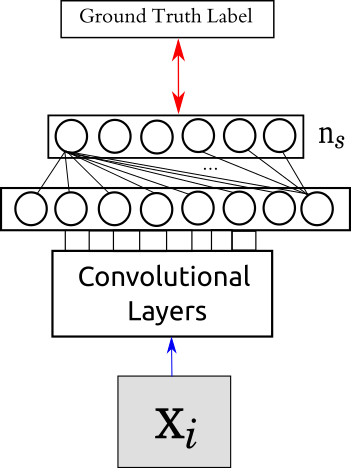
\includegraphics[scale=0.4]{hist_net}
  \caption{Proposed network architecture for mapping to histograms}
  \end{figure}
\end{frame}

% \begin{frame} \frametitle{Mapping to Histogram of Seen Classes}
%   \begin{itemize}
%     \item
%   The network  has a standard sequential architecture consisting of 17 pre-trained layers from VGG-19 and four other fully connected layers. \\
%   \item
%   Size of last layer is equal to the number of seen categories.
%   \item
%   Let $\phi$ denote the mapping modeled by the network
% \end{itemize}
% \end{frame}


\begin{frame}\frametitle{Mapping to Histogram of Seen Classes}
  \textbf{In Training Time:}
  \begin{itemize}
  \item Labeled samples from seen classes is used.
  \item Activation function in last layer is softmax:
    \begin{equation}
\label{softmax}
softmax(\mathbf{z})_j = \frac{e^{\mathbf{z}_j}}{\sum_k e^{\mathbf{z}_k}}, \quad j = 1, \ldots, n_s.
\end{equation}
  \item Training criteria is correct label prediction of labeled samples.
  \item   Let $\phi$ denote the mapping modeled by the network
  \begin{equation}
  \minimize_{\phi} \sum_{i=1}^{N_s} \sum_{j=1}^{n_s} (\mathbf{y}i)_j \times log(\phi(\mathbf{x}_i)_j) + (1- (\mathbf{y}i)_j) \times log(1 - \phi(\mathbf{x}_i)_j)
\end{equation}
\end{itemize}
\end{frame}

\begin{frame}\frametitle{Mapping to Histogram of Seen Classes}
  \textbf{In Test Time:}
\begin{itemize}
  \item Activation function in last layer is \textit{temprature softmax}:
    \begin{equation}
    \label{softmax}
    softmax_T(\mathbf{z})_j = \frac{e^{\mathbf{z}_j}/T}{\sum_k e^{\mathbf{z}_k}/T}, \quad T>1,  \quad j = 1, \ldots, n_s.
    \end{equation}
\item The softmax layer is trained to produce distribution of true label which is a discrete delta function.
\item When setting $T > 1$ the output becomes smoother.
\end{itemize}
\begin{figure}
\hfill
\subfigure[$T=1$]{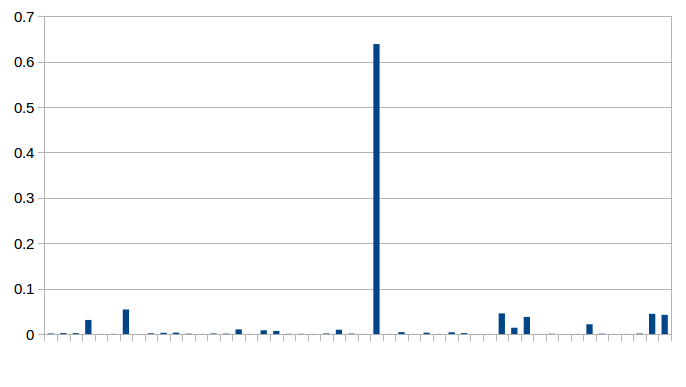
\includegraphics[width=4cm]{softmax}}
\hfill
\subfigure[$T=10$]{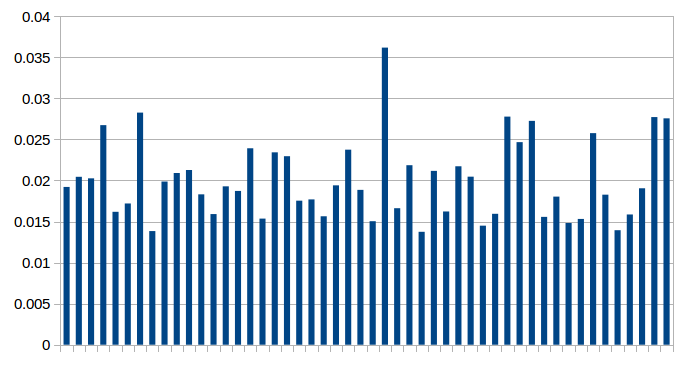
\includegraphics[width=4cm]{tsoftmax}}
\hfill
\end{figure}
\end{frame}


\begin{frame} \frametitle{Mapping to Histogram of Seen Classes}
  \begin{itemize}
    \item Singanures are mapped to space of histogram by similarity of their signatures to signature of seen classes:
    \begin{equation}
   \theta_j(\mathbf{c}) = \frac{1}{\norm{\mathbf{c - c_j}}_2  }, \quad j=1,\ldots, n_s.
   \end{equation}
   \item finally prediction can be done using nearest neighbor (or our proposed compatibility function)
\end{itemize}
\end{frame}

%


\subsection{Independent Embedding and Clustering (IEaC)}
\label{sub:Custering and Linear Embedding}
\begin{frame}\frametitle{Independent Embedding and Clustering (IEaC)}
  \textbf{Observation:}  There is a clustering structure in image space \\
  when features are extracted using Deep CNNs.
  \begin{figure}
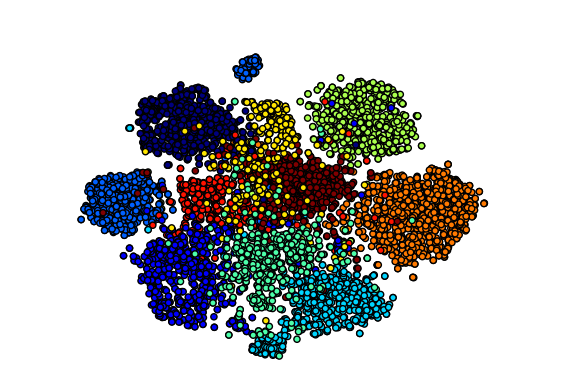
\includegraphics[width=6cm]{awa_clusters}
\caption{\scriptsize Samples of unseen classes from AwA dataset. Classes are shown in colors.}
  \end{figure}
\end{frame}

\begin{frame}\frametitle{Independent Embedding and Clustering (IEaC)}
  Motivated by this observation we propose a novel compatibility function for zero-shot learning:
  \begin{enumerate}
    \item Cluster test samples.
    \item Assign each cluster to an unseen class.
    \item All items in a cluster inherit the label received by cluster
  \end{enumerate}
  We have used two variation for the second step:
  \begin{itemize}
    \item Classify all samples and then use majority vote:
    \\ used on output of two previous methods.
    \item Classify just cluster centers.
    \\ we will present a method for this type.
  \end{itemize}
\end{frame}



\begin{frame}\frametitle{Independent Embedding and Clustering (IEaC)}
To assing label to cluster centers $\mu_k$ we propose:
\begin{itemize}
  \item Embed class signatures to image space using linear mapping $D$ from:
  \begin{equation} \label{eq:d_definition}
  D = \argmin_D \normf{X_s - D Z_s}^2 + \alpha \normf{D}^2.
\end{equation}
$X_s$: matrix of train samples, $Z_s$ true attribute vector for samples in $X_s.$
\item Assign each $\mu_k$ to an unseen class using:
\begin{equation}
\label{eq:simple_assignment}
\ell(\boldsymbol{\mu_k}) = \argmin_{u=1,\ldots,n_u} \normf{\boldsymbol{\mu_k} - D\mathbf{c}_{u}}^2
\end{equation}\end{itemize}
\end{frame}




\subsection{Joint Embedding and Clustering (JEaC)}
\label{sec:Joint Embedding and Clustering (JEaC)}

\begin{frame}\frametitle{Joint Embedding and Clustering (JEaC)}
In the previous method:
\begin{itemize}
  \item Classification Accuracy is bottlenecked by the clustering accuracy.
  \item Separate learning mapping and mapping prevents information flow.
  \item Each one is learned with a different criteria
\end{itemize}
To over come this shortcomings, we propose a \textit{Joint Embedding and Clustering} method.
\end{frame}
\begin{frame}\frametitle{Joint Embedding and Clustering}
The method is formulated as:
\begin{align}
\label{eq:joint}
 \min_{R,D} \normf{X_s - D Z_s}^2  &+ \lambda \normf{X_u - D C_u R^T }^2 + \eta \normf{D}^2, \\
   s.t. \quad & R \in \{0,1\}^{N_u \times n_u}. \nonumber
\end{align}
\begin{itemize}
  \item
  The first term is same as in Eq. \eqref{eq:d_definition}.
  \item
  The second term is essentially a clustering criteria. this will be more clear if re-written as:
  \[
  \label{eq:essentialy_clustering}
\sum_{n=N_s+1}^{N_s + N_u} \sum_{k=1}^{n_u} r_{nk} \normtwo{\mathbf{x_n} - D \mathbf{c_k}}.
  \]
\end{itemize}
\end{frame}

\section{Experimental Results}
\label{sec:Experimental Results}

\begin{frame}\frametitle{Experimental Results}
  \begin{center}
  {\scriptsize
  \begin{tabular}{|l|c|c|c|c|}
  \hline
  method  & AwA & CUB-2011 & aPY & SUN \\
  \hline

    {\tiny \cite{li15max}}                 &  $38.2 \pm 2.3$   &    -             &  -                       & $18.9 \pm 2.5$ \\
   {\tiny \cite{semi15}}                    &  $40.05\pm 2.25$ &       -          &   $24.71 \pm 3.19$       & -    \\
  \hline
   {\tiny \cite{Akata2015}}              & $66.7$          & $50.1$            &         -                & -\\
  %& {Changpinyo \textit{et al.}}~\cite{Synthesized}       & $72.9$           & $54.5$            &                         & $62.7$ \\
   {\tiny \cite{Xian2016}}                & $71.9$            & $45.5$            &        -                 & -\\
  \hline
  {\tiny \cite{Kodirov2015}}
                                              & $73.2$            &  $39.5$           & $26.5$                    &  -\\
   {\tiny \cite{Akata2015}}              & $61.9$            &  $50.1$           &                 -        & -\\
    {\tiny \cite{sse}}            &  $76.33 \pm 0.53$ & $30.41 \pm 0.20$ &   $46.23 \pm 0.53$      & $82.50 \pm 1.32$    \\
   {\tiny \cite{agnostic} }      &  $80.46 \pm 0.53$ & $42.11 \pm 0.55$ &   \textbf{$\mathbf{50.35 \pm 2.97}$}      & \underline{$83.83 \pm 0.29$}    \\
    {\tiny proposed (mapping to histograms)}
                          & $76.50 \pm 1.02$               & $33.29 \pm 0.21$              & $47.46 \pm 0.31$              & $79.88 \pm 0.42$ \\
   {\tiny proposed( IEaC -  {k-means})}
                            & $86.34 \pm 0.13$               & $52.48 \pm 0.60$              & $48.03 \pm 1.56$              & $75.75 \pm 1.06$ \\
   {\tiny proposed (IEaC - semisupervised)}
                          & \underline{$86.38 \pm 0.56$}              & \underline{$ 53.10\pm 0.43 $}             & $48.52 \pm 0.29$              &$ 80.66 \pm 0.76$ \\
   {\tiny proposed (JEaC- init D)}
                       & $83.03$                        & $57.55$                       & $42.62$          & $72.50$\\
   {\tiny roposed (JEaC - init R)}
                       & \textbf{\em $\mathbf{88.64 \pm 0.04}$}  & \textbf{\em $\mathbf{58.80 \pm 0.64}$} &
                       \underline{$49.77 \pm 2.02$} & \textbf{\em $\mathbf{86.16 \pm 0.57}$} \\
  \hline
  \end{tabular}
  }
\end{center}

\end{frame}

\subsection{Discussion}
\label{sub:Discussion}


\begin{frame}\frametitle{Demonstrating on Real Data}
\begin{figure}
  \hfill
  \subfigure[{\tiny seen/unseen}]{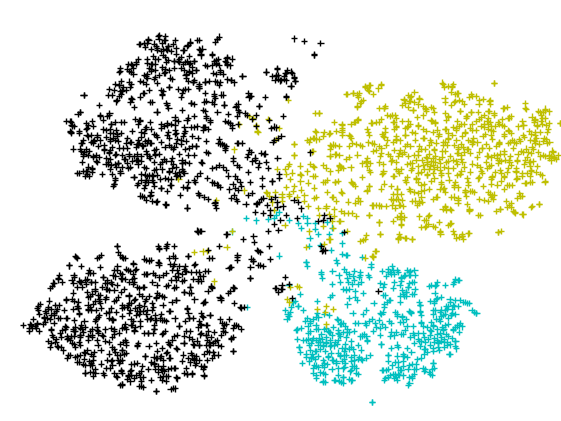
\includegraphics[width=3cm]{none}}
  \hfill
  \subfigure[{\tiny ground truth}]{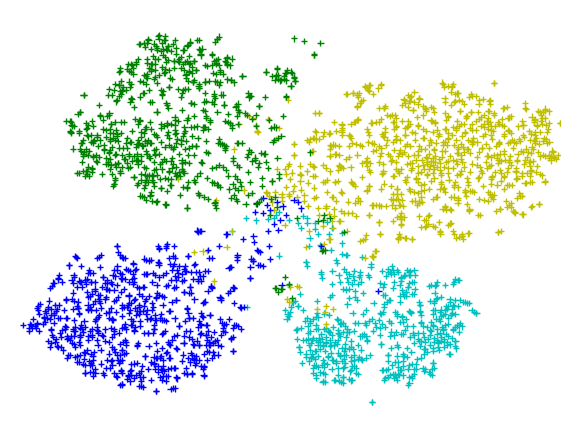
\includegraphics[width=3cm]{truth}}
  \hfill
  \subfigure[{\tiny nearest neighbor compabtibility}]{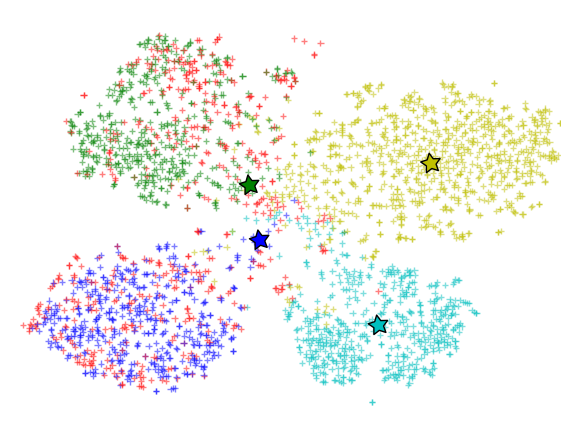
\includegraphics[width=3cm]{knn}}
  \hfill
  \subfigure[{\tiny IEaC (k-means)}]{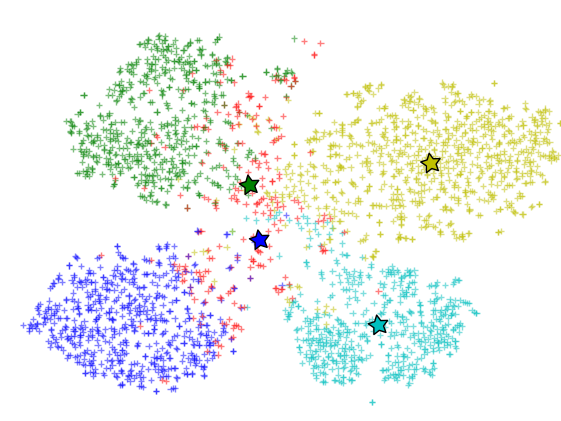
\includegraphics[width=3cm]{kmeans}}
  \hfill
  \subfigure[{\tiny IEaC (semi-supervised)}]{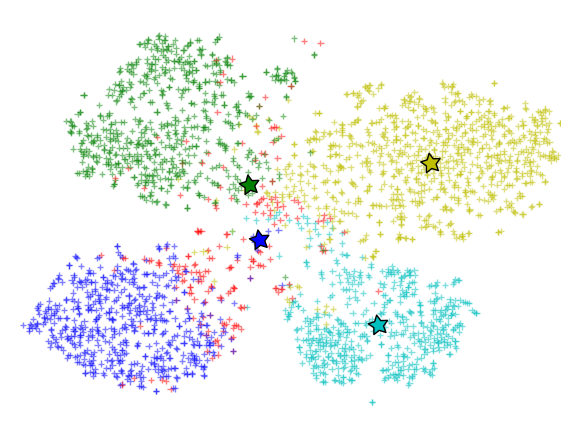
\includegraphics[width=3cm]{own_cluster}}
  \hfill
  \subfigure[{\tiny JEaC}]{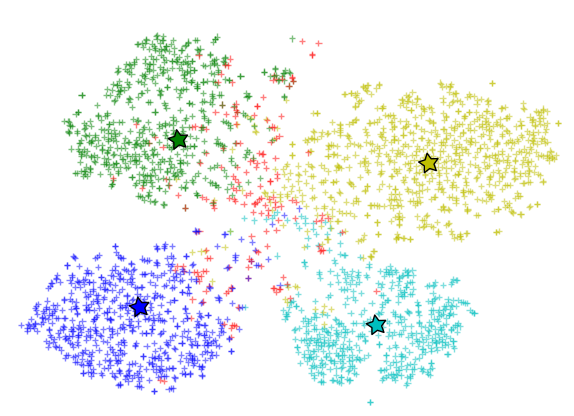
\includegraphics[width=3cm]{jeac}}
  \hfill
\end{figure}
\end{frame}

\begin{frame}
  \frametitle{Conclusion}
  In this presentation we:
  \begin{itemize}
    \item introduced the problem of zero-shot learning
    \item categorized and reviewed a selection on prior works
    \item proposed a Deep Neural network to predict attributes from images.
    \item proposed a Deep Neural network to map images to histogram of seen classes
    \item proposed a novel compatibility function and semi-supervised algorithm for zero-shot learning.
    \item used above propositions in an Independent Embedding and Clustering method
    \item extended our Independent Embedding and Clustering to do this steps jointly.
    \item Demonstrated performance of our methods through experiments.
    \item Discussed effect of different parts in our models by experimenting on a real dataset.
  \end{itemize}
\end{frame}
\begin{frame}[allowframebreaks]
        \frametitle{References}
        {\footnotesize
        \bibliographystyle{apalike}
        \bibliography{references.bib}
        }
\end{frame}

\begin{frame}[noframenumbering]\frametitle{A Sermi-Supervised Clustering Algorithm}
  Performance of proposed compatibility function depends on clustering.\\
  We present a semi-supervised clustering algorithm matching assumptions of zero-shot Learning. \\
  Formulated with an Optimization Problem:
  \begin{equation} \label{eq:my_clustering}
\min_{R, \boldsymbol{\mu_1, \ldots, \mu_k }} \sum_{n=1}^{N_s + N_u}  \sum_{k} r_{nk} \normtwo{\mathbf{x_n} - \boldsymbol{\mu_k}} +
 \beta \sum_{n=1}^{N_s} \mathds{1}(\mathbf{r_n} \neq \mathbf{y_n}).
\end{equation}
The first term is inherited from k-means clustering \\
\vspace{1mm}
The second term produces a penalty of $\beta$ if a labeled instance from seen classes
is assigned to cluster with different number.
\end{frame}


\begin{frame}[noframenumbering]\frametitle{Experimental Results for Clustering}
  \begin{table}[ht]
  \centering
    \label{tab:clustering}
    {\scriptsize
  \begin{tabular}{|r|c|c|c|c|}
  \hline
method & AwA & CUB-2011 & aPY & SUNA \\
  \hline
  k-means                             &  ${65.93 \pm 1.73}$                 & ${34.48 \pm 1.00}$           & ${65.37 \pm 3.73 }$               & ${16.83 \pm 0.76 }$   \\
  \hline
{\tiny Proposed semi-supervised clustering}
                        & \textbf{${70.74\pm 0.32}$}  & \textbf{${42.63\pm 0.07}$} & \textbf{${69.93\pm 3.40}$} & \textbf{ ${45.50 \pm 1.32}$} \\
  \hline
  \end{tabular}
  }
  \vspace{2mm}
  \end{table}
\end{frame}


\begin{frame}[noframenumbering]\frametitle{Plug Proposed Compatibility Function to other methos}
  \begin{table}[t]
\caption{Results for Multi-task Neural Network using two different compatibility functions}
\label{tab:nn_comp}
\begin{center}
  {\footnotesize
\begin{tabular}{|r|c|c|c|c|}
\hline
  & AwA & CUB-2011 & aPY & SUNA \\
\hline
Nearest Neighbor
 %                     & {${73.77}$}  & {${32.52}$} & ${33.10}$ & { ${66.50}$} \\ \hline
                & {${74.52 \pm 1.93}$}  & {${33.91 \pm 0.21}$} & ${33.10 \pm 1.36}$ & { ${66.13 \pm 0.50}$} \\ \hline
Proposed Compatibility
                      & $74.68 \pm 0.73$  & \textbf{${33.92 \pm 0.07}$} & \textbf{${38.26 \pm 1.27}$} & \textbf{ ${67.50 \pm 0.00}$} \\ \hline
\end{tabular}
}
\end{center}
\end{table}
\end{frame}


\begin{frame}\frametitle{Discussion}
  In IEaC:
  \begin{itemize}
    \item Using proposed clustering function based on clustering performs better than nearest neighbor compatibility.
    \item This is by taking in account the  unsupervised information available in images space.
  \end{itemize}
  In JEaC:
  \begin{itemize}
    \item Keeps Strong points in IEaC
    \item Jointly learning cluster assignments and linear mapping improves results.
    \item Considers good clustering while learning the mapping.
    \item Considers proximity of cluster centers and mapping of signatures while assigning clusters.
    \item This mitigates Domain-shift problem
  \end{itemize}
\end{frame}

\end{document}
